\documentclass[11pt,a4paper]{article}

% --- Packages ---
\usepackage[utf8]{inputenc}
\usepackage{amsmath}
\usepackage{graphicx} % Required for inserting images
\usepackage{booktabs}
\usepackage{hyperref}
\usepackage{geometry}
\usepackage{titlesec}

% --- Page Setup ---
\geometry{margin=1in}
\hypersetup{
    colorlinks=true,
    linkcolor=blue,
    filecolor=magenta,      
    urlcolor=cyan,
    pdftitle={Dual-Axis Solar Tracker Report},
}

% --- Title Block ---
\title{\textbf{Simplified Dual-Axis Solar Tracker Using Arduino and LDRs} \\ Term Project for Embedded Systems Laboratory EE39004}
\author{
    Group 5:
    Satyam Awasthi (16EE10042)
    Sanskar Agrawal (16EE10041)
    }
\date{April 9 2019}

\begin{document}

\maketitle

% --- Image Preview Area ---
\begin{figure}[h!]
    \centering
    % Replace 'solar-tracker-preview' with your actual image file name (e.g., .jpg or .png) uploaded to Overleaf
    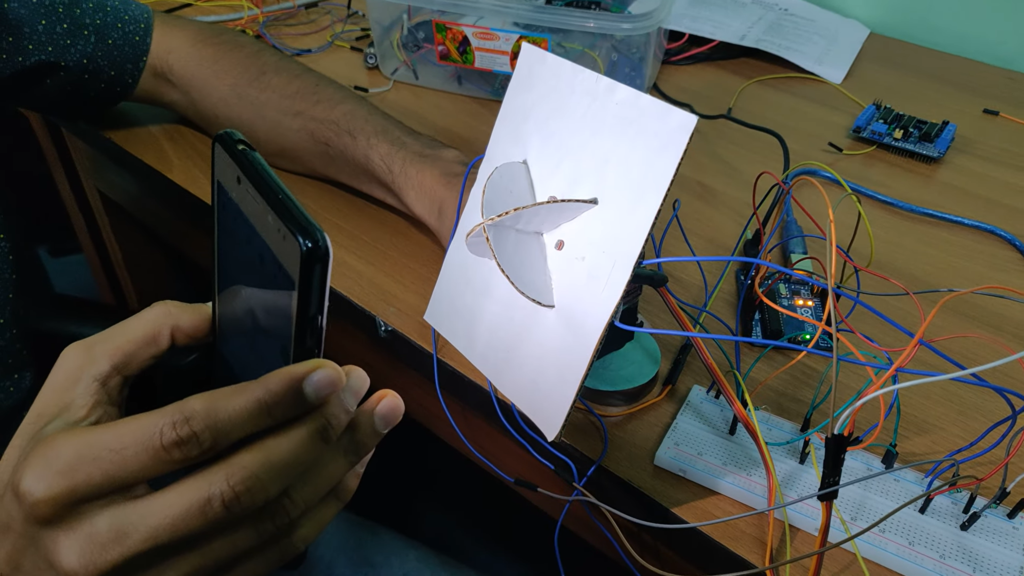
\includegraphics[width=0.7\textwidth]{7.png} 
    \caption{Prototype Preview: Dual-Axis Solar Tracking System}
    \label{fig:top_preview}
\end{figure}

\begin{abstract}
Solar trackers automatically position objects at an optimal angle relative to the Sun. While traditionally used to keep photovoltaic (PV) panels perpendicular to the Sun's rays for maximum energy absorption, they are also used to position space telescopes and heliostat mirrors. This project implements a low-cost Dual-Axis Solar Tracker using an Arduino microcontroller and Light Dependent Resistors (LDRs). The system functions as a mechanical Maximum Power Point Tracker (MPPT) designed to enhance the efficiency of solar PV systems.
\end{abstract}

\vfill
\textsf{\small \noindent \textbf{Keywords:} Arduino Uno, Solar Tracking, Photovoltaic Panels, LDR Sensors, MPPT}
\newpage

% --- Section 1: Introduction ---
\section{Introduction \& Problem Statement}
Standard solar tracking systems often rely on complex mathematical algorithms and heavy computation to maximize power output. This high level of complexity increases production costs and makes maintenance difficult for small-scale applications. 

Our project proposes a simplified mechanical solution. By using real-time light differentials captured by LDR sensors, the system dynamically adjusts two perpendicularly mounted servo motors to keep the solar panel facing the brightest light source, bypassing the need for complex tracking calculations.

% --- Section 2: Materials ---
\section{Materials and Equipment}
The components utilized to construct the prototype are detailed in Table~\ref{tab:materials} below.

\begin{table}[h!]
\centering
\caption{System Component List}
\label{tab:materials}
\begin{tabular}{lcl}
\toprule
\textbf{Component} & \textbf{Quantity} & \textbf{Purpose} \\
\midrule
Arduino Uno & 1 & System microcontroller and processing unit \\
LDR Sensors & 4 & Light intensity detection across two axes \\
Servo Motors & 2 & Actuators for horizontal and vertical movement \\
10k$\Omega$ Resistors & 4 & Voltage dividers for analog sensor readings \\
Breadboard \& Jumpers & 1 Set & Prototype circuit assembly \\
Custom Mounts & 2 & Cost-effective structural support \\
\bottomrule
\end{tabular}
\end{table}

% --- Section 3: Methodology ---
\section{Methodology and System Logic}
The system operates on a continuous feedback loop based on the difference in light energy received by four sensors arranged in a cross pattern: Top, Bottom, Left, and Right. Two servo motors provide two degrees of freedom.

\begin{verbatim}
                    [ Top LDR ]


                         |
          [ Left LDR ] --+-- [ Right LDR ]
                         |
                   [ Bottom LDR ]
\end{verbatim}

\subsection{Horizontal Tracking (Left / Right)}
The Arduino reads the analog values from the Left and Right LDRs. If the Right LDR detects a higher light intensity (lower resistance), the horizontal servo rotates right by a small angle increment. This loop repeats until the difference between the two sensor values falls below a predefined threshold.

\subsection{Vertical Tracking (Top / Bottom)}
Similarly, the vertical servo adjusts the pitch up or down based on the light differential between the Top and Bottom LDRs. The panel achieves equilibrium once the light values balance across both sensors.

\noindent The complete source code for this implementation can be reviewed at the project's repository link: \url{https://github.com/satyam-aw/Simplified-Solar-Panel-for-PV-Panels}.

% --- Section 4: Results ---
\section{Experimental Results}
A smartphone torch was used to simulate the movement of the Sun during testing. The tracker successfully followed the light source smoothly across both axes within the servo motor's structural limit of $0^\circ$ to $180^\circ$ of motion. 

\noindent A video demonstrating the operational prototype can be accessed via the following link: \url{https://youtu.be/oxEElFv9_Wo?si=fT7BZxVwzBm61ZjW}.

% --- Section 5: Challenges ---
\section{Challenges and Engineering Insights}
\begin{itemize}
    \item \textbf{Servo Rotation Limits:} Servo motors are physically restricted to a $0^\circ$ to $179^\circ$ range. The software variable controlling the angle was initialized to $90^\circ$. Conditional boundary constraints were implemented in the code to ensure the target variable never drops below $0^\circ$ or exceeds $180^\circ$.
    \item \textbf{Wire Strain:} Rapid panel movements during early tests caused jumper wires to pull loose from the breadboard. For a permanent deployment, soldering the connections is required to ensure system reliability.
    \item \textbf{Cost Optimization:} To minimize expenditures, structural servo mounts were custom fabricated by hand instead of purchasing pre-made commercial brackets.
\end{itemize}

% --- Section 6: Conclusion ---
\section{Conclusion and Future Scope}
This project successfully demonstrates that a low-cost, mechanical solar tracker can effectively complement or back up electrical MPPT systems. By maintaining a perpendicular orientation to the sun, the system maximizes energy absorption. 

The underlying sensor-driven tracking logic developed here can be easily adapted for other engineering applications, including:
\begin{enumerate}
    \item \textbf{Wind and Hydro Turbines:} Dynamic blade pitch angle control.
    \item \textbf{Telecommunications:} Automated dish antenna positioning for optimized signal reception.
\end{enumerate}

\end{document}
